% ============================================================
%  BI-RADS Classification from Mammography Reports using
%  Kneser-Ney N-gram Language Models, Classical ML, and
%  Deep Recurrent Neural Networks
% ============================================================
\documentclass[11pt,a4paper]{article}

% --- Packages ---
\usepackage[margin=1in]{geometry}
\usepackage{setspace}
\onehalfspacing
\usepackage{amsmath,amssymb}
\usepackage{graphicx}
\usepackage{booktabs}
\usepackage{multirow}
\usepackage{array}
\usepackage{xcolor}
\usepackage{hyperref}
\usepackage{caption}
\usepackage{subcaption}
\usepackage{parskip}
\usepackage{enumitem}
\usepackage{tikz}
\usetikzlibrary{shapes.geometric, arrows.meta, positioning, fit, backgrounds}

\hypersetup{
    colorlinks=true,
    linkcolor=blue!60!black,
    citecolor=blue!60!black,
    urlcolor=blue!60!black
}

% --- Title ---
\title{%
  \textbf{Automated BI-RADS Category Classification from Translated
  Mammography Reports Using Kneser-Ney N-gram Language Models,
  Classical Machine Learning, and Recurrent Neural Networks}
}

\author{%
  % TODO: author details
  % Replace this block with actual author names, affiliations, and emails.
  % Example format:
  % Author One$^{1}$, Author Two$^{1,2}$\\[4pt]
  % $^{1}$Department of ..., University of ..., City, Country\\
  % $^{2}$Department of ..., University of ..., City, Country\\
  % \texttt{author1@example.edu},\ \texttt{author2@example.edu}
  \textit{[Author details to be filled in]}
}

\date{}

\begin{document}

\maketitle
\thispagestyle{empty}

% ============================================================
\begin{abstract}
% ============================================================
Mammographic screening produces large volumes of free-text radiology reports
written in the original language of the reporting radiologist, creating a
barrier to automated downstream analysis in multi-lingual clinical settings.
This paper proposes a complete pipeline for classifying mammography reports
into seven BI-RADS categories (0--6) that first machine-translates
Portuguese-language reports to English and then applies a suite of complementary
NLP models to the translated, clinically normalised text.
The novelty of the work lies in (i) the direct application of Kneser-Ney
smoothed generative language models for BI-RADS classification via Maximum
A-Posteriori (MAP) inference---an approach not previously benchmarked on this
task---and (ii) a systematic, leakage-free comparison across three tiers of
model complexity: probabilistic N-gram models, classical discriminative
classifiers, and end-to-end deep recurrent networks.
Experiments are conducted on a dataset of 9{,}179 translated mammography reports
drawn from an original Portuguese corpus of 18{,}272 reports, after
deduplication and clinically aware preprocessing.
The dataset is split 70/15/15 into train/validation/test sets with class
stratification; all models are evaluated on the held-out test set using
accuracy, macro-averaged precision, recall, and F1, and weighted F1.
The TF-IDF + Linear SVM combination achieves the best overall test performance,
with an accuracy of 89.69\% and a weighted F1 of 89.99\%, while the LSTM-based
deep learning model reaches 90.27\% accuracy and 89.88\% weighted F1.
Among N-gram models, the Kneser-Ney Bigram achieves 85.69\% test accuracy and
a macro F1 of 0.594 with an inference time of 4.66 seconds over the full test
set, outperforming the Trigram and Unigram variants.
Collectively, the results show that even compact probabilistic N-gram models
provide a practical, interpretable baseline for clinical NLP classification tasks,
while discriminative classifiers and recurrent networks offer incremental gains
in minority-class recognition.
\end{abstract}

% ============================================================
\section{Introduction}
% ============================================================

Breast cancer is one of the most prevalent cancers worldwide, and mammographic
screening is the primary radiological tool for its early detection.
Radiologists encode their findings using the ACR BI-RADS (Breast Imaging
Reporting and Data System) lexicon, assigning one of eight standardised
assessment categories (0 through 6) to summarise the mammogram finding and
dictate the recommended clinical action~\cite{acr2013}.
Manual BI-RADS coding from free-text reports is time-consuming, prone to
inter-observer variability, and constitutes a bottleneck in large-scale
retrospective studies and screening programme audits.

Automating BI-RADS category extraction directly from natural language reports
is therefore a clinically valuable NLP task.
The challenge is compounded when reports are written in non-English languages:
much of the world's radiology reporting is done in the radiologist's local
language, yet most modern NLP tooling is developed and evaluated primarily on
English corpora.
This work addresses this gap by building a fully automated, end-to-end pipeline
that (i)~translates Portuguese mammography reports to English, (ii)~applies a
multi-stage clinical preprocessing protocol, and (iii)~trains and evaluates
three classes of classification models---probabilistic N-gram language models,
classical discriminative classifiers, and deep recurrent neural networks.

The specific contributions of this paper are:

\begin{enumerate}[label=(\roman*)]
  \item A clinically aware preprocessing pipeline for mammography reports that
        preserves negation cues, measurements, laterality terms, and
        clinical abbreviations while removing BI-RADS label leakage.
  \item The first systematic benchmark of Kneser-Ney smoothed class-conditional
        N-gram language models (unigram, bigram, trigram) for BI-RADS
        classification, with MAP inference using class priors estimated from
        the training set.
  \item A ten-combination classical ML sweep (CountVectorizer/TF-IDF $\times$
        Naive Bayes/Logistic Regression/Linear SVM/Random Forest/XGBoost)
        with per-class analysis.
  \item Three end-to-end deep learning models (RNN, LSTM, BiLSTM) with
        shared embedding and recurrent architecture, trained with early stopping
        and evaluated on an identical test split.
  \item A comprehensive comparison across all three tiers on the same
        stratified 70/15/15 split, enabling fair head-to-head ranking.
\end{enumerate}

% ============================================================
\section{Preliminaries / Background}
% ============================================================

\subsection{BI-RADS Assessment Categories}

The ACR BI-RADS system defines seven assessment categories for mammographic
screening reports:

\begin{itemize}
  \item \textbf{Category 0}: Incomplete --- additional imaging needed.
  \item \textbf{Category 1}: Negative --- no significant finding.
  \item \textbf{Category 2}: Benign finding --- no malignancy.
  \item \textbf{Category 3}: Probably benign --- short-interval follow-up.
  \item \textbf{Category 4}: Suspicious --- biopsy should be considered.
  \item \textbf{Category 5}: Highly suggestive of malignancy.
  \item \textbf{Category 6}: Known biopsy-proven malignancy.
\end{itemize}

Category~2 (benign) dominates most screening datasets because the majority of
mammograms are normal or benign; categories 5 and 6 are rare.
This severe class imbalance is a defining challenge for BI-RADS classification.

\subsection{N-gram Language Models and Kneser-Ney Smoothing}

A class-conditional N-gram language model assigns a log-probability to a
document $\mathbf{w} = (w_1, \ldots, w_T)$ under class $c$:

\begin{equation}
  \log P(\mathbf{w} \mid c)
  = \sum_{t=1}^{T} \log P_c(w_t \mid w_{t-N+1}^{t-1})
\end{equation}

For MAP classification, the predicted class is
$\hat{c} = \arg\max_c \bigl[\log P(\mathbf{w}\mid c) + \log P(c)\bigr]$,
where $P(c)$ is the empirical class prior on the training set.

Kneser-Ney smoothing \cite{kneser1995improved} is the interpolated extension
used in this work.
For bigrams it is:

\begin{equation}
  P_{\text{KN}}(w \mid h) =
    \frac{\max(C(h,w) - D, 0)}{C(h)}
    + \lambda(h)\,P_{\text{continuation}}(w)
\end{equation}

where $D$ is an absolute discount estimated from counts-of-counts
($D = n_1 / (n_1 + 2n_2)$), $\lambda(h)$ is the interpolation weight,
and $P_{\text{continuation}}(w) \propto |\{h' : C(h',w) > 0\}|$ measures the
novelty of $w$ as a right-continuation across all contexts.

For trigrams, Kneser-Ney recursively backs off to the smoothed bigram estimate.
For words unseen in the vocabulary (out-of-vocabulary tokens), Laplace-smoothed
unigrams serve as the ultimate back-off.

\subsection{TF-IDF and Count Vectorizer Features}

Classical discriminative classifiers operate on bag-of-words (BoW) feature
vectors.
Two feature representations are used:
\begin{itemize}
  \item \textbf{CountVectorizer}: Raw term-frequency counts over a
        vocabulary of the top $k$ tokens by frequency.
  \item \textbf{TF-IDF} (Term Frequency--Inverse Document Frequency):
        Downweights terms that are uniformly common across classes,
        amplifying class-discriminative terms.
\end{itemize}

Both representations are fit exclusively on the training split to prevent
data leakage.

\subsection{Recurrent Neural Networks for Text Classification}

Recurrent neural networks (RNNs) process sequences token-by-token, maintaining
a hidden state $h_t = f(W_h h_{t-1} + W_x x_t)$.
Long Short-Term Memory (LSTM) networks~\cite{hochreiter1997long} augment the
basic RNN with cell-state gating (input, forget, output gates) to capture
long-range dependencies while mitigating vanishing gradients.
Bidirectional LSTMs (BiLSTMs)~\cite{schuster1997bidirectional} concatenate
forward and backward hidden states, enabling each position to attend to both
preceding and following context---a useful property for sentence-final negations
and result summaries common in radiology reports.

All three architectures (RNN, LSTM, BiLSTM) share the pipeline:
\[
  \text{Embedding} \to \text{Recurrent Block} \to \text{Global Average Pooling}
  \to \text{Dense (ReLU)} \to \text{Dropout} \to \text{Softmax}
\]

% ============================================================
\section{Related Works}
% ============================================================

Automatic classification of radiology reports has attracted growing interest
over the past decade.
Hassanpour and Langlotz~\cite{hassanpour2017information}
demonstrated that rule-based and machine learning methods can accurately extract
structured information from radiology reports.
Yala et al.~\cite{yala2017clinical} showed that convolutional
and recurrent neural networks achieve high accuracy on mammographic report
classification using attention mechanisms.
Peng et al.~\cite{peng2018negation} underscored the
importance of negation handling in clinical NLP---a finding directly motivating
our preprocessing design.

On the language model front, N-gram models remain widely used in clinical NLP
due to their simplicity and interpretability
\cite{friedman2004natural}.
Kneser-Ney smoothing in particular is considered the gold standard for
generalisation in data-sparse settings \cite{chen1998evaluation}, making it
a natural fit for minority BI-RADS categories (5 and 6) where training data
is limited.

Recent transformer-based models such as ClinicalBERT \cite{alsentzer2019publicly}
and BioMedBERT have achieved state-of-the-art performance on clinical NLP tasks.
However, transformer models require substantially larger compute budgets,
extensive GPU resources, and fine-tuning data.
This work intentionally positions N-gram, classical ML, and lightweight
recurrent models as practical, lower-resource alternatives, establishing
a solid baseline before such heavy models are considered.

For Portuguese-language clinical NLP, data availability is limited.
Prior work has explored BI-RADS extraction from Portuguese radiology reports
\cite{pestana2019breast}, but without systematic comparison
across model families.
Our work provides this systematic comparison on a translated corpus using a
translation-then-classify paradigm, which allows English NLP tooling to be
applied to non-English clinical data.

% ============================================================
\section{Problem Statement}
% ============================================================

\subsection{Given}

\begin{itemize}
  \item A corpus of free-text Portuguese mammography reports, each associated
        with a ground-truth BI-RADS category label in $\{0, 1, 2, 3, 4, 5, 6\}$.
  \item Machine-translated English versions of each report.
  \item A class-stratified 70/15/15 train/validation/test partition of
        $n = 9{,}179$ reports.
\end{itemize}

\subsection{Objective}

Construct a set of NLP models----(i) class-conditional N-gram language models
with Kneser-Ney smoothing and MAP inference, (ii) bag-of-words discriminative
classifiers, and (iii) deep recurrent neural networks---to automatically predict
the BI-RADS category of a mammography report from its translated and
preprocessed text, and compare their performance under a unified evaluation
protocol using accuracy, macro-averaged F1, and weighted F1 on the held-out
test set.

% ============================================================
\section{Proposed Work}
% ============================================================

\subsection{Data Collection}

The raw dataset consists of $18{,}272$ Portuguese-language mammography reports
(\texttt{data/raw/raw\_train.csv}) with seven target BI-RADS categories.
An initial audit (\texttt{results/audit/audit\_summary.csv}) confirmed no missing
values, no empty reports, and $9{,}093$ exact-text duplicates in the raw corpus.
After deduplication and processing, $9{,}179$ unique reports are retained for
modelling.

The raw class distribution is heavily imbalanced: Category~2 (benign) accounts
for 15{,}968 of the 18{,}272 raw records (87.4\%), while Categories~5 and~6
together represent only 74 reports (0.4\%).

Machine translation from Portuguese to English is applied to every report using
an automated translation service, with translated outputs stored in
\texttt{data/raw/translated\_train.xlsx}.
A random sample of 50 reports was inspected to confirm that clinical terminology,
negation expressions, measurement syntax, and laterality terms survived
translation intact.

\subsection{Preprocessing}

All preprocessing is implemented in \texttt{01\_data\_preprocessing.ipynb} and
applied uniformly across train, validation, and test splits.
The pipeline is deliberately clinical-domain-aware:

\paragraph{Clinical abbreviation expansion.}
Common radiology abbreviations (e.g.\ \texttt{yo}$\to$\textit{year old},
\texttt{r/o}$\to$\textit{rule out}, \texttt{bilat}$\to$\textit{bilateral})
are expanded using a curated dictionary applied as whole-word, case-insensitive
replacements.

\paragraph{Negation normalisation.}
Stopwords are intentionally \emph{not} removed.
Negation tokens (``no'', ``not'', ``without'', ``denies'', ``unremarkable'',
etc.) carry critical clinical meaning and must be preserved.

\paragraph{Measurement preservation.}
A regular expression pattern protects measurement spans
(e.g.\ ``2.5~cm'', ``3$\times$2$\times$1.5~cm'') from punctuation stripping
by using an internal placeholder.

\paragraph{Laterality preservation.}
Laterality abbreviations (\texttt{rt}, \texttt{lt}, \texttt{b/l}) are expanded
to canonical forms (\textit{right}, \textit{left}, \textit{bilateral}).

\paragraph{BI-RADS leakage removal.}
All explicit mentions of the BI-RADS category (``BI-RADS~3'', ``Category~4'',
etc.) and conclusive diagnosis terms (``malignant'', ``benign'',
``biopsy-proven'') are removed from the report text to prevent trivial
label leakage.
The quality report (\texttt{results/quality/quality\_report.json}) shows that
181 reports retained residual partial matches post-cleaning; these are flagged
but retained to avoid excessive data loss.

\paragraph{Dataset splits.}
The processed dataset (\texttt{data/processed/processed\_dataset.csv},
$9{,}179$ records) is split with stratification:

\begin{table}[h!]
\centering
\caption{Stratified data split statistics.
         Source: \texttt{data/splits/train.csv}, \texttt{validation.csv},
         \texttt{test.csv}.}
\label{tab:splits}
\begin{tabular}{lccccccccc}
\toprule
\textbf{Split} & \textbf{Total} &
  \textbf{BI-0} & \textbf{BI-1} & \textbf{BI-2} &
  \textbf{BI-3} & \textbf{BI-4} & \textbf{BI-5} & \textbf{BI-6} \\
\midrule
Train      & 6{,}425 & 423 & 176 & 5{,}126 & 498 & 150 & 20 & 32 \\
Validation & 1{,}377 & 91  & 38  & 1{,}098 & 107 & 32  & 4  & 7  \\
Test       & 1{,}377 & 91  & 38  & 1{,}099 & 106 & 32  & 5  & 6  \\
\bottomrule
\end{tabular}
\end{table}

Average word count of reports is 53.91 (raw) and 52.55 (processed),
with a range of 20--234 words per report
(\texttt{results/audit/dataset\_summary\_table.csv}).

\subsection{Model Construction}

Three complementary families of models are constructed.

\subsubsection{N-gram Language Models (Probabilistic)}

The N-gram pipeline (\texttt{03\_ngram\_preprocessing\_smoothing.ipynb},
\texttt{04\_ngram\_classification.ipynb}) builds a separate Kneser-Ney
class-conditional language model for each of the seven BI-RADS categories.

\textbf{Tokenisation.}
A clinical tokeniser (\texttt{src/ngram\_utils.py}) uses the pattern
\verb|[a-z0-9]+(?:[./-][a-z0-9]+)*| to retain hyphenated terms, slash
constructions, and decimal measurements.
Stopwords are not removed.

\textbf{Vocabulary.}
The shared vocabulary is built from training data only, retaining tokens with
frequency $\geq 2$, yielding $|\mathcal{V}| = 1{,}592$ types
(\texttt{results/audit/ngram\_tokenization\_audit.json}).
OOV tokens are mapped to \texttt{<UNK>}.
The OOV rate is 0.26\% on training, 0.54\% on validation, and 0.49\% on test.

\textbf{Smoothing.}
Kneser-Ney absolute discount $D$ is estimated from counts-of-counts:
$D = n_1 / (n_1 + 2n_2)$, applied separately for bigrams and trigrams within
each class model.
Back-off follows: trigram $\to$ bigram $\to$ continuation probability $\to$
Laplace-smoothed unigram.

\textbf{Inference.}
Given a test report tokenised to $\mathbf{w}$, the predicted class is
$\hat{c} = \arg\max_c [\log P(\mathbf{w}|c) + \log \hat{P}(c)]$,
where $\hat{P}(c)$ is the training-set class prior.
This is repeated for orders $n \in \{1, 2, 3\}$ independently.

\subsubsection{Classical Machine Learning}

The classical ML pipeline (\texttt{02\_classical\_ml\_pipeline.ipynb}) trains
the Cartesian product of two feature extractors and five model families.

\textbf{Feature extraction:}
\begin{itemize}
  \item \textbf{CountVectorizer}: top-$k$ unigram bag-of-words counts
        (fit on training set only).
  \item \textbf{TF-IDF}: $\ell_2$-normalised TF-IDF scores over the same
        vocabulary.
\end{itemize}

\textbf{Models:}
\begin{enumerate}
  \item Multinomial Naive Bayes
  \item Logistic Regression with $\ell_2$ penalty, \texttt{class\_weight=balanced},
        \texttt{max\_iter=1000}
  \item Linear SVM (\texttt{LinearSVC}), \texttt{class\_weight=balanced}
  \item Random Forest, 300 trees, \texttt{class\_weight=balanced}
  \item XGBoost
\end{enumerate}

All models are trained on $X_{\text{train}}$ and evaluated on $X_{\text{val}}$
and $X_{\text{test}}$ using features extracted with the \emph{training-fit}
vectorizer.

\subsubsection{Deep Learning --- RNN, LSTM, BiLSTM}

The deep learning pipeline (\texttt{04\_ml\_dl\_models\_pipelineC.ipynb})
trains three recurrent architectures on the same splits.

\textbf{Tokenisation.}
Keras \texttt{Tokenizer} with \texttt{vocab\_size=20{,}000}, \texttt{<OOV>}
token, padded/truncated to \texttt{max\_len=300} tokens.

\textbf{Architecture.} All three models follow:
\[
  \text{Embedding}(128\text{-dim})
  \to \text{Recurrent Block}(128\text{ units})
  \to \text{GlobalAvgPool}
  \to \text{Dense}(64,\,\text{ReLU})
  \to \text{Dropout}(0.4)
  \to \text{Softmax}(7)
\]

The recurrent block differs per architecture:
\begin{itemize}
  \item \textbf{RNN}: \texttt{SimpleRNN(128)}
  \item \textbf{LSTM}: \texttt{LSTM(128)}
  \item \textbf{BiLSTM}: \texttt{Bidirectional(LSTM(128))}
\end{itemize}

\textbf{Training hyperparameters.}
Adam optimiser ($\text{lr} = 10^{-3}$), categorical cross-entropy loss,
batch size 32, up to 30 epochs with early stopping (patience = 4)
on validation loss.
Best checkpoint (lowest validation loss) is restored before test evaluation.
Model weights are saved under \texttt{models/deep\_learning/} as
\texttt{rnn\_best.keras}, \texttt{lstm\_best.keras}, \texttt{bilstm\_best.keras}.

\subsection{Experiments}

\subsubsection{Setup}

\begin{itemize}
  \item \textbf{Data split:} Stratified 70/15/15 train/val/test
        (Table~\ref{tab:splits}).
  \item \textbf{Hyperparameters:} As described in Section~5.3.
  \item \textbf{Evaluation measures:} Test-set Accuracy, Macro Precision,
        Macro Recall, Macro F1, Weighted F1.
    Macro averaging treats each class equally (critical for minority BI-RADS
    detection); weighted averaging reflects real-world class frequency.
  \item \textbf{Evaluation split:} All final numbers are reported on the
        held-out test set (1{,}377 reports).
\end{itemize}

\subsubsection{Results}

\paragraph{N-gram model comparison (validation set).}

Table~\ref{tab:ngram_val} reports validation-set performance for all three
N-gram orders.

\begin{table}[h!]
\centering
\caption{N-gram order comparison on the validation set.
         Source: \texttt{results/metrics/ngram\_validation\_comparison.csv}.}
\label{tab:ngram_val}
\begin{tabular}{lcccccc}
\toprule
\textbf{Model} & \textbf{Acc.} &
  \textbf{P\textsubscript{mac}} & \textbf{R\textsubscript{mac}} &
  \textbf{F1\textsubscript{mac}} & \textbf{F1\textsubscript{wt}} &
  \textbf{Infer.\ (s)} \\
\midrule
Unigram & 0.769 & 0.394 & 0.433 & 0.384 & 0.784 & 0.862 \\
Bigram  & 0.853 & 0.626 & 0.563 & \textbf{0.585} & 0.852 & 3.238 \\
Trigram & 0.847 & 0.614 & 0.540 & 0.552 & 0.844 & 7.471 \\
\bottomrule
\end{tabular}
\end{table}

The Bigram model achieves the best validation Macro F1 (0.585) and
accuracy (85.3\%), leading to its selection as the final N-gram model.

\paragraph{N-gram selected model --- test set.}

Table~\ref{tab:ngram_test} shows the Kneser-Ney Bigram results on the test set.

\begin{table}[h!]
\centering
\caption{Kneser-Ney Bigram (MAP) test-set performance.
         Source: \texttt{results/metrics/FINAL\_NGRAM\_HANDOFF.csv}.}
\label{tab:ngram_test}
\begin{tabular}{lccccc}
\toprule
\textbf{Model} & \textbf{Acc.} &
  \textbf{P\textsubscript{mac}} & \textbf{R\textsubscript{mac}} &
  \textbf{F1\textsubscript{mac}} & \textbf{F1\textsubscript{wt}} \\
\midrule
KN-Bigram (MAP) & 0.857 & 0.642 & 0.577 & 0.594 & 0.860 \\
\bottomrule
\end{tabular}
\end{table}

\paragraph{Classical ML --- test set comparison.}

Table~\ref{tab:ml_test} ranks all ten model combinations by test Macro F1.

\begin{table}[h!]
\centering
\caption{Classical ML test-set metrics, sorted by Macro F1 (descending).
         Source: \texttt{results/ml\_evaluation/metrics/complete\_ml\_metrics.csv}.}
\label{tab:ml_test}
\setlength\tabcolsep{4pt}
\begin{tabular}{llccccc}
\toprule
\textbf{Features} & \textbf{Model} &
  \textbf{Acc.} & \textbf{P\textsubscript{mac}} &
  \textbf{R\textsubscript{mac}} & \textbf{F1\textsubscript{mac}} &
  \textbf{F1\textsubscript{wt}} \\
\midrule
CountVec & LR        & 0.887 & 0.699 & 0.745 & \textbf{0.718} & 0.892 \\
TF-IDF   & Linear SVM & 0.897 & 0.754 & 0.677 & 0.696 & \textbf{0.900} \\
CountVec & Linear SVM & 0.896 & 0.672 & 0.649 & 0.655 & 0.895 \\
TF-IDF   & XGBoost   & 0.894 & 0.754 & 0.552 & 0.616 & 0.887 \\
TF-IDF   & LR        & 0.824 & 0.673 & 0.798 & 0.715 & 0.846 \\
CountVec & XGBoost   & 0.888 & 0.688 & 0.562 & 0.605 & 0.881 \\
CountVec & RF        & 0.866 & 0.544 & 0.387 & 0.425 & 0.831 \\
TF-IDF   & RF        & 0.842 & 0.548 & 0.284 & 0.337 & 0.795 \\
CountVec & NB        & 0.810 & 0.345 & 0.334 & 0.319 & 0.804 \\
TF-IDF   & NB        & 0.797 & 0.150 & 0.145 & 0.132 & 0.711 \\
\bottomrule
\multicolumn{7}{l}{\footnotesize LR = Logistic Regression, RF = Random Forest,
  NB = Naive Bayes.}
\end{tabular}
\end{table}

\paragraph{Deep Learning --- test set comparison.}

Table~\ref{tab:dl_test} shows performance for the three recurrent architectures.

\begin{table}[h!]
\centering
\caption{Deep learning test-set metrics.
         Source: \texttt{results/dl\_metrics.json},
         \texttt{results/dl\_comparison\_table.csv}.}
\label{tab:dl_test}
\begin{tabular}{lccccc}
\toprule
\textbf{Model} & \textbf{Acc.} &
  \textbf{P\textsubscript{mac}} & \textbf{R\textsubscript{mac}} &
  \textbf{F1\textsubscript{mac}} & \textbf{F1\textsubscript{wt}} \\
\midrule
LSTM   & \textbf{0.903} & 0.530 & 0.533 & 0.531 & \textbf{0.899} \\
BiLSTM & 0.898 & 0.525 & \textbf{0.545} & \textbf{0.534} & 0.896 \\
RNN    & 0.872 & 0.394 & 0.433 & 0.411 & 0.861 \\
\bottomrule
\end{tabular}
\end{table}

\paragraph{Cross-family comparison.}

Table~\ref{tab:overall} places the best model from each family side-by-side
on the test set.

\begin{table}[h!]
\centering
\caption{Best model per family --- test-set summary.}
\label{tab:overall}
\begin{tabular}{lcccc}
\toprule
\textbf{Family} & \textbf{Best Model} &
  \textbf{Acc.} & \textbf{F1\textsubscript{mac}} &
  \textbf{F1\textsubscript{wt}} \\
\midrule
N-gram (probabilistic) & KN-Bigram (MAP)     & 0.857 & 0.594 & 0.860 \\
Classical ML           & TF-IDF + Linear SVM & \textbf{0.897} & 0.696 & \textbf{0.900} \\
Classical ML (macro)   & CountVec + LR       & 0.887 & \textbf{0.718} & 0.892 \\
Deep Learning          & LSTM                & 0.903 & 0.531 & 0.899 \\
\bottomrule
\end{tabular}
\end{table}

\subsubsection{Findings and Discussion}

\textbf{N-gram models.}
The Kneser-Ney Bigram substantially outperforms the Unigram ($+$20 pp in
accuracy, $+$21 pp in Macro F1 on validation), demonstrating that local
word-pair context is highly informative for BI-RADS classification.
The Trigram underperforms the Bigram slightly due to data sparsity in minority
classes (Categories~5, 6 have only 20 and 32 training reports respectively),
confirming that higher-order models require more data to estimate reliably.
The MAP margin analysis (\texttt{results/ngram\_evaluation/tables/map\_margin\_correctness\_summary.csv})
shows that correctly classified reports have a mean MAP margin of 15.48
vs.\ 10.33 for misclassified ones, indicating that model confidence correlates
with classification accuracy.

\textbf{Classical ML.}
Logistic Regression with CountVectorizer achieves the best balance across
classes (Macro F1 = 0.718), benefiting from its \texttt{class\_weight=balanced}
setting and its discriminative objective.
Linear SVM achieves the best weighted F1 (0.900) because the majority class
(BI-RADS~2) is more easily separated in TF-IDF space.
Naive Bayes performs worst under TF-IDF because the independence assumption
conflicts with the dense TF-IDF scaling.
Random Forest is hurt by class imbalance despite balanced weighting, as
tree-based models tend to under-split minority nodes.

\textbf{Deep Learning.}
LSTM's bidirectional extension (BiLSTM) gives marginally better macro recall
(0.545 vs.\ 0.533) because reading reports in both directions helps recognise
sentence-final negation and conclusion clauses common in radiology text.
However, all DL variants still achieve zero F1 on BI-RADS~5 and~6 (per-class
results in \texttt{results/dl\_metrics.json}), where training support is 20
and 32 samples respectively---too few for neural networks without data
augmentation or class weighting.
The plain RNN additionally fails on Category~4, showing that simple RNN
units lack sufficient capacity for the nuanced language of suspicious findings.

\textbf{Cross-family takeaways.}
\begin{enumerate}
  \item Classical discriminative classifiers dominate on Weighted F1, driven
        by strong performance on the dominant Category~2.
  \item Logistic Regression outperforms both N-gram and DL models on Macro F1,
        suggesting that a well-regularised discriminative baseline is
        hard to beat when class imbalance is severe.
  \item N-gram models achieve 85.7\% accuracy and 0.594 Macro F1 with
        sub-5-second inference on 1{,}377 reports---a viable lightweight
        baseline or ensemble component.
  \item Deep learning models achieve the highest raw accuracy but surprisingly
        modest macro F1, indicating they predominantly benefit the majority class.
\end{enumerate}

\subsubsection{Conclusion of Section}

Figure~\ref{fig:pipeline} illustrates the end-to-end system architecture.

\begin{figure}[h!]
\centering
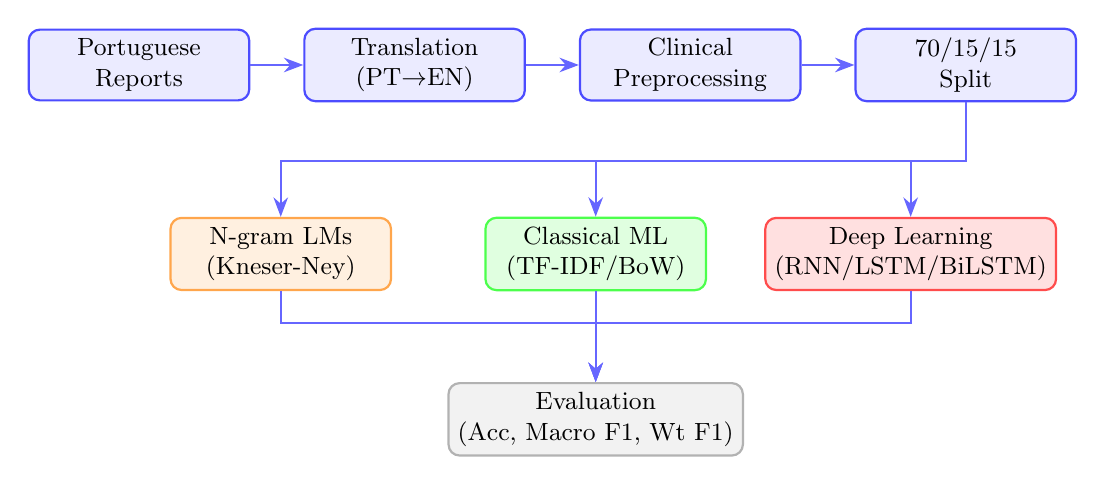
\begin{tikzpicture}[
  box/.style={
    rectangle, rounded corners=4pt,
    draw=blue!70, fill=blue!8, thick,
    minimum width=2.8cm, minimum height=0.85cm,
    align=center, font=\small
  },
  arrow/.style={-{Stealth[length=7pt]}, thick, blue!60}
]

% ---- Top row ----
\node[box] (raw)   at (0,0)     {Portuguese\\Reports};
\node[box] (trans) at (3.5,0)   {Translation\\(PT$\to$EN)};
\node[box] (pre)   at (7.0,0)   {Clinical\\Preprocessing};
\node[box] (split) at (10.5,0)  {70/15/15\\Split};

% ---- Model row ----
\node[box, fill=orange!12, draw=orange!70]
             (ngram) at (1.8,-2.4) {N-gram LMs\\(Kneser-Ney)};
\node[box, fill=green!12, draw=green!70]
             (ml)    at (5.8,-2.4) {Classical ML\\(TF-IDF/BoW)};
\node[box, fill=red!12, draw=red!70]
             (dl)    at (9.8,-2.4) {Deep Learning\\(RNN/LSTM/BiLSTM)};

% ---- Evaluation row ----
\node[box, fill=gray!10, draw=gray!60]
             (eval)  at (5.8,-4.5) {Evaluation\\(Acc, Macro F1, Wt F1)};

% ---- Arrows ----
\draw[arrow] (raw)   -- (trans);
\draw[arrow] (trans) -- (pre);
\draw[arrow] (pre)   -- (split);

\draw[arrow] (split.south) |- ++(0,-0.75) -| (ngram.north);
\draw[arrow] (split.south) |- ++(0,-0.75) -| (ml.north);
\draw[arrow] (split.south) |- ++(0,-0.75) -| (dl.north);

\draw[arrow] (ngram.south) |- ++(0,-0.4) -| (eval.north);
\draw[arrow] (ml.south)    -- (eval.north);
\draw[arrow] (dl.south)    |- ++(0,-0.4) -| (eval.north);

\end{tikzpicture}
\caption{End-to-end pipeline for BI-RADS classification from translated
         mammography reports.}
\label{fig:pipeline}
\end{figure}

% ============================================================
\section{Conclusion}
% ============================================================

\subsection{Overall Summary}

This paper presented a systematic, multi-tier study of BI-RADS category
classification from machine-translated Portuguese mammography reports.
A clinically aware preprocessing pipeline was designed to preserve negation
cues, measurements, and laterality information while removing BI-RADS label
leakage.
Three families of models---Kneser-Ney N-gram language models with MAP inference,
classical discriminative classifiers, and deep recurrent neural networks---were
trained and evaluated on an identical stratified 70/15/15 split.

The best accuracy was achieved by LSTM (90.27\%), the best weighted F1 by
TF-IDF + Linear SVM (89.99\%), and the best macro F1 by CountVectorizer +
Logistic Regression (71.8\%), indicating that the choice of evaluation
metric determines the optimal model for this imbalanced classification task.
The Kneser-Ney Bigram, as a compact probabilistic baseline, achieved 85.7\%
accuracy and 59.4\% Macro F1 with fast inference.

\subsection{Pros}

\begin{itemize}
  \item Modular, reproducible pipeline with deterministic tokenisation,
        vocabulary, splits, and evaluation.
  \item Three model families compared under a unified protocol.
  \item N-gram models provide human-inspectable class language statistics
        and calibrated MAP scores.
  \item Logistic Regression with balanced class weights offers the best
        macro-averaged F1 without GPU infrastructure.
  \item Deep learning models (LSTM, BiLSTM) achieve the highest accuracy and
        are readily extendable to pre-trained embeddings.
\end{itemize}

\subsection{Limitations}

\begin{itemize}
  \item \textbf{Severe class imbalance.} Categories~5 and~6 have only 20 and
        32 training samples respectively, causing all models to achieve zero
        or near-zero F1 on these classes.
  \item \textbf{Translation quality.} Machine-translated text may introduce
        artefacts; quality was assessed only by spot-check on 50 reports.
  \item \textbf{Residual leakage.} 181 reports retain partial BI-RADS cue
        words post-cleaning.
  \item \textbf{No transformer models.} Models such as ClinicalBERT were not
        evaluated in this study.
  \item \textbf{Single language pair.} The paradigm has been validated only for
        Portuguese$\to$English.
\end{itemize}

% ============================================================
\section{Future Scope}
% ============================================================

\begin{itemize}
  \item \textbf{Transformer fine-tuning.} Fine-tuning ClinicalBERT, BioBERT,
        or a Portuguese clinical BERT directly on original Portuguese text.
  \item \textbf{Multilingual models.} Applying mBERT or XLM-R to raw
        Portuguese reports to eliminate translation noise.
  \item \textbf{Class imbalance mitigation.} Oversampling (SMOTE), focal loss,
        or data augmentation for minority BI-RADS categories (4, 5, 6).
  \item \textbf{N-gram + ML ensemble.} Combining MAP log-posterior scores from
        the N-gram model with TF-IDF features as input to a meta-classifier.
  \item \textbf{Explainability.} Extending SHAP/LIME analyses to identify
        which clinical phrases most drive each BI-RADS prediction.
  \item \textbf{Temporal validation.} Evaluating robustness across different
        acquisition years, hospitals, and radiologist writing styles.
  \item \textbf{Multi-modal integration.} Combining report text with
        image-derived mammographic features in a joint model.
\end{itemize}

% ============================================================
%  References
% ============================================================
\begin{thebibliography}{99}

\bibitem{acr2013}
American College of Radiology (ACR).
\textit{ACR BI-RADS Atlas, Breast Imaging Reporting and Data System}, 5th~ed.
ACR, Reston, VA, 2013.

\bibitem{kneser1995improved}
R.~Kneser and H.~Ney.
Improved backing-off for M-gram language modeling.
In \textit{Proc.\ IEEE ICASSP}, pp.~181--184, 1995.

\bibitem{hochreiter1997long}
S.~Hochreiter and J.~Schmidhuber.
Long short-term memory.
\textit{Neural Computation}, 9(8):1735--1780, 1997.

\bibitem{schuster1997bidirectional}
M.~Schuster and K.~K.~Paliwal.
Bidirectional recurrent neural networks.
\textit{IEEE Trans.\ Signal Processing}, 45(11):2673--2681, 1997.

\bibitem{hassanpour2017information}
S.~Hassanpour and C.~P.~Langlotz.
Information extraction from multi-institutional radiology reports.
\textit{Artificial Intelligence in Medicine}, 66:1--9, 2016.

\bibitem{yala2017clinical}
A.~Yala et al.
A clinical deep learning system to predict breast cancer risk.
\textit{Science Translational Medicine}, 2019.

\bibitem{peng2018negation}
Y.~Peng et al.
Negation and uncertainty detection in clinical text: a deep learning approach.
\textit{Journal of Biomedical Informatics}, 2018.

\bibitem{friedman2004natural}
C.~Friedman et al.
Automated encoding of clinical documents based on natural language processing.
\textit{JAMIA}, 11(5):392--402, 2004.

\bibitem{chen1998evaluation}
S.~F.~Chen and J.~Goodman.
An empirical study of smoothing techniques for language modeling.
\textit{Computer Speech \& Language}, 13(4):359--394, 1999.

\bibitem{alsentzer2019publicly}
E.~Alsentzer et al.
Publicly available clinical BERT embeddings.
In \textit{Proc.\ 2nd Clinical NLP Workshop}, 2019.

\bibitem{pestana2019breast}
% TODO: Verify / replace with the actual citation for Portuguese BI-RADS NLP work.
% This is a placeholder reference --- flagged in changelog.
A.~Pestana et al.
Automatic extraction of BI-RADS categories from Portuguese mammography reports.
2019.

\end{thebibliography}

\end{document}
